\documentclass[nofonts]{ctexart}
\usepackage[colorlinks, linkcolor=black,CJKbookmarks]{hyperref}
\usepackage{graphicx}
\usepackage[left=2.5cm,right=2.5cm,top=2.5cm,bottom=2.5cm]{geometry}
\usepackage{indentfirst}
\usepackage{boxedminipage}
\usepackage{tikz}

\setCJKmainfont[ItalicFont={STFangsong}]{SimSun}
\setCJKsansfont{WenQuanYi Zen Hei}
\setCJKmonofont{AR PL UKai CN}

\CTEXsetup[titleformat=\sf,format={\raggedright \large}]{section}

\begin{document}
\sloppy

\title{
  远程在线嵌入式系统实验教学与探索
}
\author{方元\\ \ \small 南京大学电子科学与工程学院}
\date{\today}
\maketitle

\setlength{\parindent}{2em}

\begin{center} \begin{minipage}[t]{.8\textwidth}
\tt \baselineskip=4pt
\setlength\parindent{2em}\Large
\abstract{电子工程类的嵌入式系统课程配套实验。
本实验基于PXA270
实验平台,讨论Qt的移植问题。(30--50字)}\\
{\bf 关键词:GUI、QTOPIA、PXA270}
\end{minipage}
\end{center}

\section{背景}
    自上世纪末以来,随着计算机技术的发展及产业化应用需求的不断扩大,嵌入式系统
应用发展极为迅猛,经过十多年的发展,嵌入式系统在我们今天的日常生活中已经随处
可见。为满足社会的需求,本世纪初,国内各高校电子类专业纷纷开设了嵌入式系统
课程,并配有相应的实验。初期的嵌入式系统实验主要围绕 ARM7 嵌入式内核,进行
bootloader 和 uC/OS--II 操作系统移植,以及在 uC/OS--II 上进行应用程序设计。
最近几年,由于处理器性能的不断提高,嵌入式系统实验内容已经开始逐渐向更高级的
操作系统演变,课程内容的深度和广度都在不断增加。

    随着国内经济的快速发展和生活水平的不断提高,电子产品的智能化趋势也相当
明显。嵌入式系统是智能电子产品的重要组成部分。目前国内人才市场急需嵌入式系统
应用开发的专业技术人才,而且缺口有逐年加大的趋势。

    与内容和难度不断增加的嵌入式系统实验不相适应的另一方面是,课程的课时并没有
增加,实验课时数和内容的矛盾日渐突出。

    与此同时,国内高校正面酝酿着实验教学改革,对开放课程、虚拟电子实验室、反转
课堂等多种手段进行积极的探索。根据《教育信息化十年发展规划(2011--2020年)》,
教育部 2013 年启动开展国家级虚拟仿真实验教学中心建设工作,虚拟仿真
实验教学的管理和共享平台是中心建设的重要内容之一。

    我们的实验系统设计正是产生于这样的背景。实验的软件部分基于嵌入式Linux
操作系统。处理器性能不再是瓶颈,而Linux社区可以提供丰富的软件资源。
学习在这个系统上进行软硬件开发可以为将来的应用建立良好的基础。

\section{实验环境的构建}

\subsection{实验系统框架}

    我们的实验平台是基于 Cortex-A8 内核的嵌入式系统。实验内容从 Linux 操作
系统移植开始,包括文件系统制作、设备驱动、图形界面、音频接口及上层应用软件
程序设计。实验硬件平台构造如图\ref{fig1}所示。主机使用Linux操作系统,并配置
了针对目标机(实验系统)平台的交叉编译工具链。主机和目标机之间通过串口和网口
连接。串口连接的作用是在目标机系统启动阶段和系统正常运行阶段对其进行监控。
图\ref{fig2}是串口软件 minicom 的配置界面,其中比较重要的参数是本机使用的
串口设备(此处设为 /dev/ttyUSB0),串行数据传输方式等。

\begin{figure}
\centering
\includegraphics[width=0.8\textwidth]{old_system}
\caption{实验系统框架}\label{fig1}
\end{figure}

\begin{figure}
\centering
\fontsize{9}{8}\selectfont
\begin{verbatim}

Welcome to minicom 2.7

    +-----------------------------------------------------------------------+
    | A -    Serial Device      : /dev/ttyUSB0                              |
    | B - Lockfile Location     : /var/lock                                 |
    | C -   Callin Program      :                                           |
    | D -  Callout Program      :                                           |
    | E -    Bps/Par/Bits       : 115200 8N1                                |
    | F - Hardware Flow Control : No                                        |
    | G - Software Flow Control : No                                        |
    |                                                                       |
    |    Change which setting?                                              |
    +-----------------------------------------------------------------------+
            | Screen and keyboard      |
            | Save setup as dfl        |
            | Save setup as..          |
            | Exit                     |
            +--------------------------+


CTRL-A Z for help | 115200 8N1 | NOR | Minicom 2.7 | VT102 | Online 0:0 | ttyUSB0              
\end{verbatim}
\caption{minicom配置界面}\label{fig2}
\end{figure}

网络连接的作用是系统启动阶段进行操作系统镜像文件的传输,以及在系统开发阶段
使用网络文件系统服务(NFS---Network File System)。

\subsection{现有实验环境的不足}
为了使学生切实掌握完整的嵌入式系统开发过程,培养学生分析问题和
解决问题的能力,我们对每个实验都没有规定最终完成的结果,而是让学生根据自己的
能力探索实验。因此,学生在实验过程中会花费比较多的时间。例如在对内核的配置
过程中,
学生在实验中需要了解应该选择哪些选项,哪些选项是可以从内核中排除的,不正确的
选项会导致什么样的后果,等等。图\ref{fig3}展示了Linux操作系统内核配置的主
菜单界面。

\begin{figure}
\centering
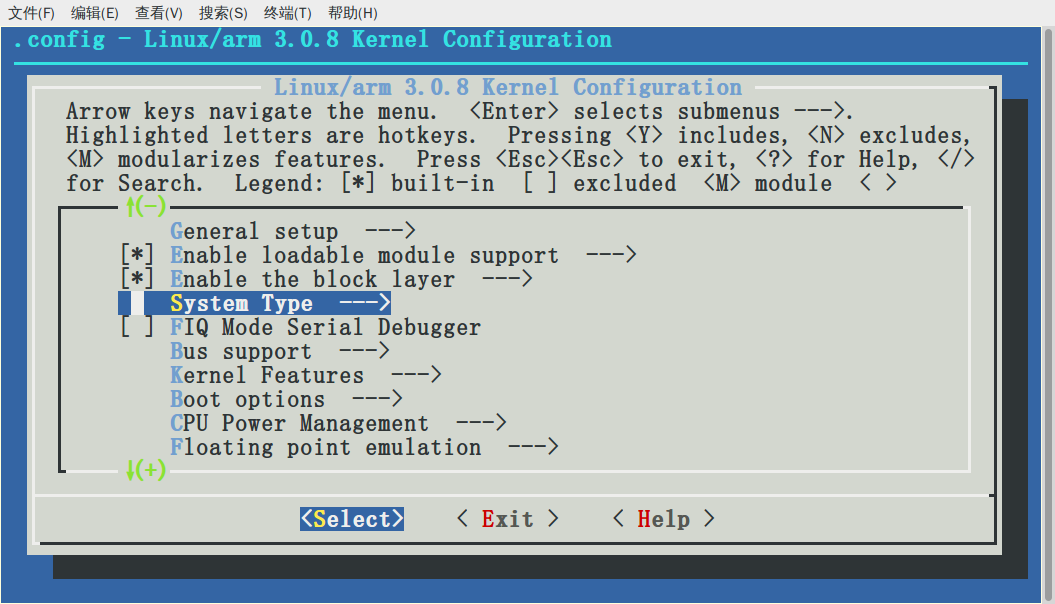
\includegraphics[width=.8\textwidth]{menu0}
\caption{Linux 内核配置主菜单}\label{fig3}
\end{figure}

理论上说每个人的结果应该是各不相同的。要完成一个正常的内核启动,
单就内核移植这一部分,即使最肤浅的做法,也很难在四个实验课时内完成(通常这套
实验课程安排不到40课时)。
并且在整理实验报告的过程中还会发现新的问题,认真的同学甚至希望回
实验室重新验证,但实验室却不总是具备这样的开放条件。

    针对这样的实验特点,我们构建了嵌入式系统的网络实验环境。网络实验除了大大
增加了学生自主支配的实验时间以外,还可以让学生在校园网的任何地方都能进行
多数的实体实验。

\section{实验内容设计}
\subsection{网络实验环境}
    Linux 操作系统自身具备的完善的内置网络功能,为我们构建网络实验环境提供了
良好的基础。

    实验系统由位于实验中心的网络实验室和可联网的个人计算机终端两部分组成。
网络实验室的一台服务器为每一套实验设备开设一个虚拟机,并为每个虚拟机分配一个
独立的串口设备,用于监控目标系统。

\begin{figure}[!h]
\centering
\includegraphics[width=.8\textwidth]{server}
\caption{网络实验系统}\label{fig4}
\end{figure}

    学生实验时,可使用校园内联网的任何一台个人计算机通过远程访问协议登录
服务器,选择一个未被占用的虚拟机,使用 Linux 基本的字符界面功能即可在该
虚拟机对应的嵌入式目标板上进行系统的实验。

\subsection{内核和根文件系统移植}
	制作内核和根文件系统镜像是后续实验的基础。这个实验安排在整个系统实验的
前期,除了实验本身涉及知识点繁多以外,学生刚开始实验,经验也比较欠缺。编译、
调式的过程要反复多次,错误的内核镜像文件常常会导致系统死机。对于较老的内核
版本,必须通过手工断电复位。新版内核配置中,可以通过设置选项``Default panic
timeout'',让系统在一定时间无正确响应后自动重启(图\ref{fig5}),保证了远程实验
的可操作性。\footnote{实验系统具有远程控制开关,在其他一些失控的情况下仍然
允许用户远程复位。}

\begin{figure}[!h]
\centering
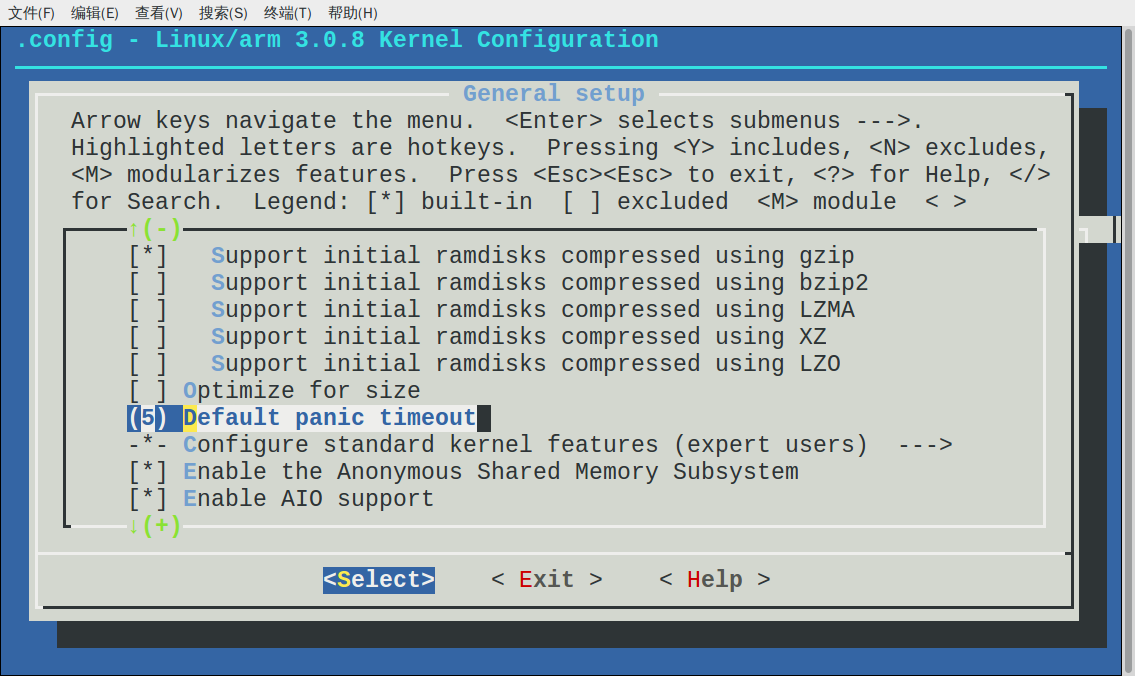
\includegraphics[width=.8\textwidth]{menu1}
\caption{内核启动异常时的自动重启选项}\label{fig5}
\end{figure}

	系统启动后一个重要的环节是给系统配置网络环境。在网络实验系统中,这项工作
至少有两个重要意义:一是在下面的实验中利用网络文件系统开发其他软件(嵌入式系统
的开发特点决定的),二是在后续实验中一旦出现串口终端失控仍可以通过 telnet 等
网络方式登录到系统继续实验,或者重启系统。

	网络配置、网络服务工作可以在系统正常启动后手工完成,也可以通过启动脚本
自动完成。自动完成的脚本内容如下(/etc/rc):

\begin{boxedminipage}{.9\textwidth}
\begin{verbatim}
#!/bin/sh
hostname EELab_03
mount -t proc proc /proc
mount -t sysfs sysfs /sys
ifconfig eth0 192.168.200.128

mount -t devpts devpts /dev/pts

telnetd -l /bin/login
\end{verbatim}
\end{boxedminipage}

其中挂载支持伪终端设备的文件系统(devpts)需要在内核配置中支持,telnetd 守护进程
在 busybox (根文件系统基本命令软件包)中支持,它们共同用来实现 Linux 系统的远程
登录。telnet 不是远程登录的唯一途径,实验中选择这种方法主要是因为比较简单,
无需图形库支持。

\subsection{嵌入式应用软件开发和测试}
	应用软件开发相对简单:在主机上交叉编译,通过网络上传/共享给目标系统,在
目标系统上运行、测试。不便之处在于,目标机在远程实验室,凡是涉及到人机交互
的地方暂时都难以实现。目前可以做到的是,在目标机中预先安装一个小软件,
用于抓取显示缓存中的数据并将其通过网络传输到主机,主机端再编写一个对应的软件
将该数据还原成图像,实现类似远程监控的功能。这两端的软件都不复杂,甚至不需要
额外编程,直接使用 busybox 中的基本命令就可以完成。

\section{不足与改进}
	在线网络实验室是实体实验室的延伸,它大大地增加了有效实验时间和自由度。
在条件允许的情况下,课时计划中的集中实验时间里,教学人员可以进行更深入
的指导和讨论,而不会再受到实验课时不足的限制。

	限于技术水平,目前的系统的最大缺点是无法实现人工操作。毕竟不是真正意义
上的虚拟实验,而是网络和实体结合的实验系统。针对系统性错误导致的目标机失控,
手工复位仍是必须的手段。对此我们也开发了专门针对本实验目标板的远程电源控制
系统,在基于权限和身份认证的前提下可以确保同时参与网络实验的学生之间不会
相互干扰。而应用程序的人机交互问题,如触摸屏实验、按键及IO设备驱动、以及
多媒体软件移植和开发实验,暂时还没有完美的解决方案。

\begin{thebibliography}{99}
\bibitem{book1}
作者.\newblock{\em 书名} ,出版社,年代时间

\end{thebibliography}

\end{document}

